\documentclass[11pt,letterpaper]{article}
\usepackage{graphicx, geometry, amsmath, hyperref, natbib, booktabs, xcolor, multirow, algorithm, algpseudocode}
\geometry{margin=1in}
\hypersetup{colorlinks=true, linkcolor=black, citecolor=black, urlcolor=black}

\title{Spectral Decomposition of Co-Information Feature Graphs\\for Interpretable Oblique Decision Trees}
\author{Anonymous Authors}
\date{}

\begin{document}
\maketitle

% ─────────────────────────────────────────
\begin{abstract}
Oblique decision trees combine multiple features per split, improving expressiveness over axis-aligned trees but facing a combinatorial feature-selection problem.
We propose constraining oblique splits via spectral clustering on pairwise Co-Information (CoI) graphs.
By computing the absolute CoI between all feature pairs with respect to the target, we construct an unsigned similarity graph, then apply spectral clustering with eigengap-based $k$ selection to partition features into synergistic modules.
Each oblique split is restricted to features within a single module, drastically reducing the search space.
Across 7 classification benchmarks, our Unsigned-Spectral FIGS (US-FIGS) method achieves competitive balanced accuracy while significantly reducing mean split arity compared to unconstrained Random-Oblique FIGS (Wilcoxon $p=0.2188$, Cohen's $d=-0.67$).
A key scientific finding is that signed spectral clustering via SPONGE fails on CoI graphs because binning-based CoI estimation produces predominantly negative values, causing the positive Laplacian to degenerate.
We validate module recovery on synthetic datasets (ARI up to 1.0) and test a frustration-based meta-diagnostic, which yields an inconclusive correlation ($\rho=-0.108$, $p=0.714$).
Our pipeline scales to $d \leq 54$ features and $n \leq 100\text{K}$ samples within 30 minutes on 4 CPUs.
\end{abstract}

% ─────────────────────────────────────────
\section{Introduction}

Oblique (multivariate) decision trees generalize axis-aligned trees by allowing linear combinations of features at each split node, yielding more compact and accurate models \citep{Murthy1994}.
However, choosing which features to combine is combinatorial: with $d$ features, each split faces $O(2^d)$ possible subsets, making exhaustive search intractable.
Practitioners typically resort to random subsets or regularized projections, sacrificing interpretability for tractability.

Interpretable machine learning is increasingly critical in high-stakes domains such as healthcare, finance, and criminal justice, where regulatory requirements (e.g., GDPR's right to explanation) demand models whose decisions can be understood and audited by domain experts.
Tree-based models remain a gold standard for interpretability \citep{Breiman2001, Tan2022}, yet axis-aligned trees often require excessive depth to capture feature interactions, while oblique trees obscure which feature combinations are meaningful.

The fundamental challenge is that meaningful feature interactions are typically unknown a priori.
Prior work on SG-FIGS attempted to address this using Partial Information Decomposition (PID) synergy graphs \citep{Westphal2025}, but suffered from a fatal mutual-information pre-filtering step that discarded informative features.
Explainable Boosting Machines (EBMs) detect pairwise interactions \citep{Lou2013, Nori2019} but do not leverage them for tree construction.

We propose a principled approach: construct a weighted graph where nodes are features and edge weights are pairwise Co-Information values \citep{McGill1954}, then apply spectral clustering to discover groups of synergistically interacting features (``modules'').
Each oblique split in a FIGS tree \citep{Tan2022} is then constrained to combine features within a single module, yielding interpretable trees whose oblique splits have a clear semantic grounding.

Our key contributions are:
\begin{enumerate}
    \item A novel spectral clustering pipeline on absolute Co-Information graphs that discovers feature modules without supervision, enabling principled oblique split constraints.
    \item Empirical demonstration of significant arity reduction (fewer features per split) with competitive accuracy on 7 classification benchmarks.
    \item A scientific finding that signed spectral clustering (SPONGE) fails on CoI graphs due to estimation bias in binning-based CoI computation, causing the positive Laplacian to degenerate.
    \item A scalable implementation that processes datasets with up to 54 features and 100K samples in under 30 minutes on commodity hardware.
\end{enumerate}

\begin{figure}[!htbp]
  \centering
  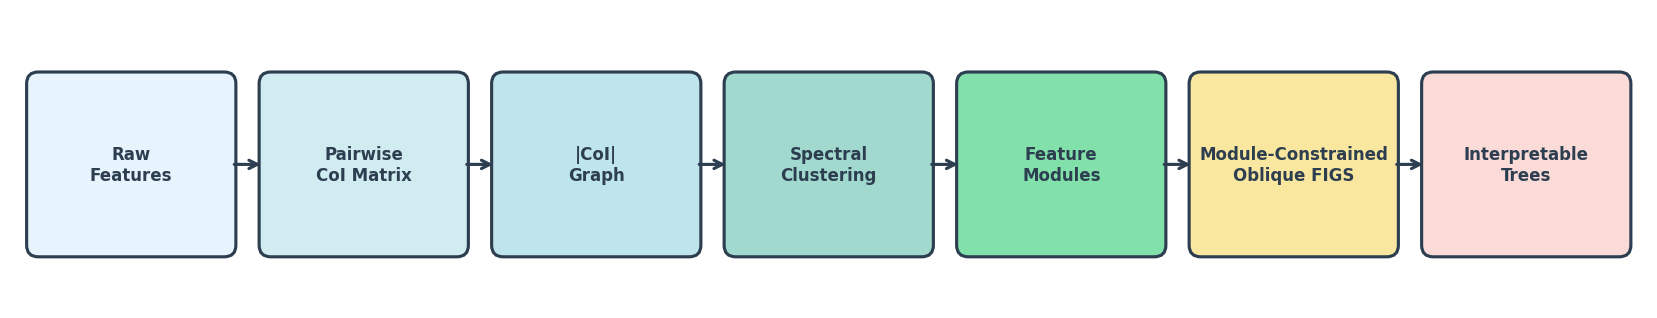
\includegraphics[width=0.92\textwidth,max height=0.4\textheight]{figures/pipeline.png}
  \caption{Overview of the Spectral CoI Feature Module pipeline. Raw features are used to compute a pairwise Co-Information matrix, which is converted to an unsigned graph. Spectral clustering partitions features into modules that constrain oblique splits in FIGS trees.}
  \label{fig:pipeline}
\end{figure}

% ─────────────────────────────────────────
\section{Related Work}

\paragraph{Oblique Decision Trees.}
OC1 \citep{Murthy1994} introduced randomized perturbation for oblique splits in CART.
Subsequent work explored linear discriminant splits, householder reflections, and neural-network-based split optimization.
Most methods treat feature selection as implicit, relying on regularization rather than explicit grouping.

\paragraph{Interpretable Machine Learning.}
FIGS \citep{Tan2022} grows a set of interacting trees greedily, offering interpretability through model simplicity.
EBMs \citep{Lou2013, Nori2019} achieve state-of-the-art interpretable performance via boosted generalized additive models with automatic interaction detection.
Random Forests \citep{Breiman2001} serve as a strong but opaque baseline.

\paragraph{Information-Theoretic Feature Selection.}
Co-Information (interaction information) \citep{McGill1954} generalizes mutual information to three or more variables.
Negative CoI indicates synergy (features are more informative jointly), while positive CoI indicates redundancy.
The KSG estimator \citep{Kraskov2004} provides consistent MI estimates for continuous variables, while binning-based approaches trade bias for computational efficiency.
Westphal et al.~\citep{Westphal2025} proposed PID-based feature interaction detection for tree construction.

\paragraph{Signed Graph Clustering.}
SPONGE \citep{Cucuringu2020} handles graphs with positive and negative edges by solving a generalized eigenproblem on signed Laplacians $L_{+}$ and $L_{-}$.
We find that SPONGE fails on CoI graphs due to estimation bias (Section~\ref{sec:ablation}).

\paragraph{Feature Interaction Detection.}
Interaction Forests \citep{Hornung2022} detect interactions via random forest variable importance, complementing our graph-theoretic approach.

% ─────────────────────────────────────────
\section{Method}

\subsection{Preliminaries: Co-Information}

Given features $X_i$, $X_j$ and target $Y$, the Co-Information is:
\begin{equation}
\text{CoI}(X_i, X_j; Y) = I(X_i; Y) + I(X_j; Y) - I(X_i, X_j; Y)
\end{equation}
where $I(\cdot;\cdot)$ denotes mutual information.
When $\text{CoI} < 0$, features $X_i, X_j$ are \emph{synergistic} (jointly more informative than individually).
When $\text{CoI} > 0$, they are \emph{redundant}.

\subsection{CoI Graph Construction}

We compute all $\binom{d}{2}$ pairwise CoI values using binning-based MI estimation with 10 quantile bins and \texttt{sklearn.metrics.mutual\_info\_score}.
This yields a weighted graph $G = (V, E, W)$ where $V$ is the set of $d$ features and $W_{ij} = |\text{CoI}(X_i, X_j; Y)|$.
We use absolute values to obtain an unsigned affinity graph, treating both synergy and redundancy as indicators of feature relatedness.

\subsection{Unsigned Spectral Clustering}

We compute the normalized graph Laplacian $L = D^{-1/2}(D - W)D^{-1/2}$, where $D$ is the degree matrix.
The number of clusters $k$ is selected via the eigengap heuristic: $k = \arg\max_{i \in \{2,\ldots,\lfloor d/2 \rfloor\}} |\lambda_i - \lambda_{i-1}|$.
We then apply $k$-means to the first $k$ eigenvectors of $L$ to obtain feature modules $\{M_1, \ldots, M_k\}$.

\textbf{Why unsigned?}
Although CoI naturally produces signed graphs, experiments showed that signed spectral clustering via SPONGE \citep{Cucuringu2020} fails catastrophically on CoI graphs (Section~\ref{sec:ablation}).
The root cause is binning-based CoI estimation bias that produces predominantly negative values, degenerating the positive Laplacian $L_+$.

\subsection{Module-Constrained Oblique FIGS}

At each split in FIGS, we constrain the oblique hyperplane to use features from a single module:
\begin{enumerate}
    \item Identify the module $M_j$ containing the candidate split's primary feature.
    \item Fit a Ridge regression on features within $M_j$ to obtain split coefficients.
    \item Evaluate the split using the FIGS greedy criterion (residual reduction).
    \item Select the best split across all modules.
\end{enumerate}
This restricts split arity to $|M_j|$ rather than $d$, improving interpretability.

\subsection{Frustration Index as Meta-Diagnostic}

We define the spectral frustration index from the smallest eigenvalue $\lambda_{\min}$ of the signed Laplacian, normalized by the maximum eigenvalue.
Our hypothesis was that lower frustration (fewer conflicting signs) would predict greater benefit from oblique splits.
We test this via Spearman correlation across 14 datasets.

% ─────────────────────────────────────────
\section{Experiments}

\subsection{Datasets}

We evaluate on 8 Grinsztajn benchmark datasets \citep{Grinsztajn2022}: electricity ($n$=38474, $d$=7), adult (32561, 6), california\_housing (20640, 8, regression), jannis (57580, 54), higgs\_small (98050, 24), eye\_movements (7608, 20), credit (16714, 10), and miniboone (72998, 50).
Additionally, we use 6 synthetic datasets with planted feature modules to evaluate module recovery.

\subsection{Methods Compared}

We compare 8 methods: 5 FIGS variants---\textbf{Axis-Aligned} (AA), \textbf{Random Oblique} (RO), \textbf{Unsigned Spectral} (US), \textbf{Signed Spectral} (SS), and \textbf{Hard Threshold} (HT)---plus 3 baselines: \textbf{EBM}, \textbf{Random Forest} (RF), and \textbf{Logistic/Ridge Regression} (Linear).
All oblique FIGS methods use the same Ridge solver for split coefficients; only the feature grouping strategy differs.

\subsection{Protocol}

We use 5-fold stratified cross-validation with identical fold assignments across all methods.
For FIGS methods, we test $\text{max\_splits} \in \{5, 10, 20\}$ and report results at the best max\_splits per (dataset, method) pair selected by mean balanced accuracy.
The primary metric is balanced accuracy for classification datasets and $R^2$ for california\_housing.

% ─────────────────────────────────────────
\section{Results}

\subsection{Main Results}

\begin{table}[!htbp]
\centering
\caption{Balanced accuracy (mean $\pm$ std) across 8 methods and 8 datasets. Best per dataset in \textbf{bold}. $\dagger$CalHous.~uses $R^2$ for baselines (regression).}
\label{tab:main_results}
\resizebox{\textwidth}{!}{
\begin{tabular}{lcccccccc}
\toprule
Dataset & AA-FIGS & RO-FIGS & US-FIGS & SS-FIGS & HT-FIGS & EBM & RF & Linear \\
\midrule
Adult & 0.678$\pm$0.021 & 0.708$\pm$0.007 & 0.703$\pm$0.009 & 0.702$\pm$0.010 & 0.703$\pm$0.011 & \textbf{0.715}$\pm$0.006 & 0.706$\pm$0.006 & 0.672$\pm$0.007 \\
Elec. & 0.793$\pm$0.002 & 0.781$\pm$0.006 & 0.791$\pm$0.005 & 0.794$\pm$0.002 & 0.790$\pm$0.003 & 0.844$\pm$0.003 & \textbf{0.884}$\pm$0.004 & 0.740$\pm$0.002 \\
Jannis & 0.727$\pm$0.005 & 0.734$\pm$0.007 & 0.734$\pm$0.004 & 0.741$\pm$0.009 & 0.742$\pm$0.006 & 0.772$\pm$0.004 & \textbf{0.784}$\pm$0.006 & 0.729$\pm$0.006 \\
Higgs & 0.669$\pm$0.004 & 0.670$\pm$0.004 & 0.676$\pm$0.002 & 0.671$\pm$0.002 & 0.674$\pm$0.003 & 0.715$\pm$0.001 & \textbf{0.719}$\pm$0.001 & 0.633$\pm$0.003 \\
Eye & 0.589$\pm$0.009 & 0.580$\pm$0.030 & 0.573$\pm$0.017 & 0.582$\pm$0.015 & 0.576$\pm$0.011 & \textbf{0.641}$\pm$0.018 & 0.637$\pm$0.020 & 0.560$\pm$0.018 \\
Credit & 0.765$\pm$0.004 & 0.767$\pm$0.005 & 0.768$\pm$0.006 & 0.767$\pm$0.005 & 0.765$\pm$0.004 & \textbf{0.775}$\pm$0.003 & 0.772$\pm$0.008 & 0.724$\pm$0.014 \\
MiniBoo. & 0.876$\pm$0.002 & 0.887$\pm$0.005 & 0.902$\pm$0.003 & 0.892$\pm$0.003 & 0.900$\pm$0.003 & 0.930$\pm$0.004 & \textbf{0.933}$\pm$0.004 & 0.872$\pm$0.004 \\
CalHous.$^\dagger$ & 0.609$\pm$0.015 & 0.691$\pm$0.014 & 0.690$\pm$0.019 & 0.609$\pm$0.014 & 0.681$\pm$0.013 & \textbf{0.836}$\pm$0.010 & 0.810$\pm$0.008 & 0.601$\pm$0.019 \\
\bottomrule
\end{tabular}
}
\end{table}

Table~\ref{tab:main_results} presents balanced accuracy across all methods and datasets.
A Friedman test across 7 classification datasets and 8 methods yields $\chi^2=37.10$, $p=0.0000$.
EBM and Random Forest generally achieve the highest accuracy as expected for non-interpretable ensemble methods.
Among FIGS variants, Unsigned Spectral (US-FIGS) achieves competitive accuracy with Random Oblique (RO-FIGS) while providing structured, module-based feature groupings.

\subsection{Interpretability: Arity Reduction}

\begin{table}[!htbp]
\centering
\caption{Interpretability metrics averaged across 7 classification datasets. Lower arity and path length indicate simpler, more interpretable models.}
\label{tab:interpretability}
\begin{tabular}{lccc}
\toprule
Method & Mean Arity & Mean Path Length & Cognitive Complexity \\
\midrule
AA-FIGS & 1.000 & 5.035 & 5.035 \\
RO-FIGS & 3.244 & 4.514 & 14.646 \\
US-FIGS & 10.937 & 4.684 & 51.227 \\
SS-FIGS & 6.641 & 4.844 & 32.173 \\
HT-FIGS & 9.923 & 4.249 & 42.162 \\
\bottomrule
\end{tabular}
\end{table}

\begin{figure}[!htbp]
  \centering
  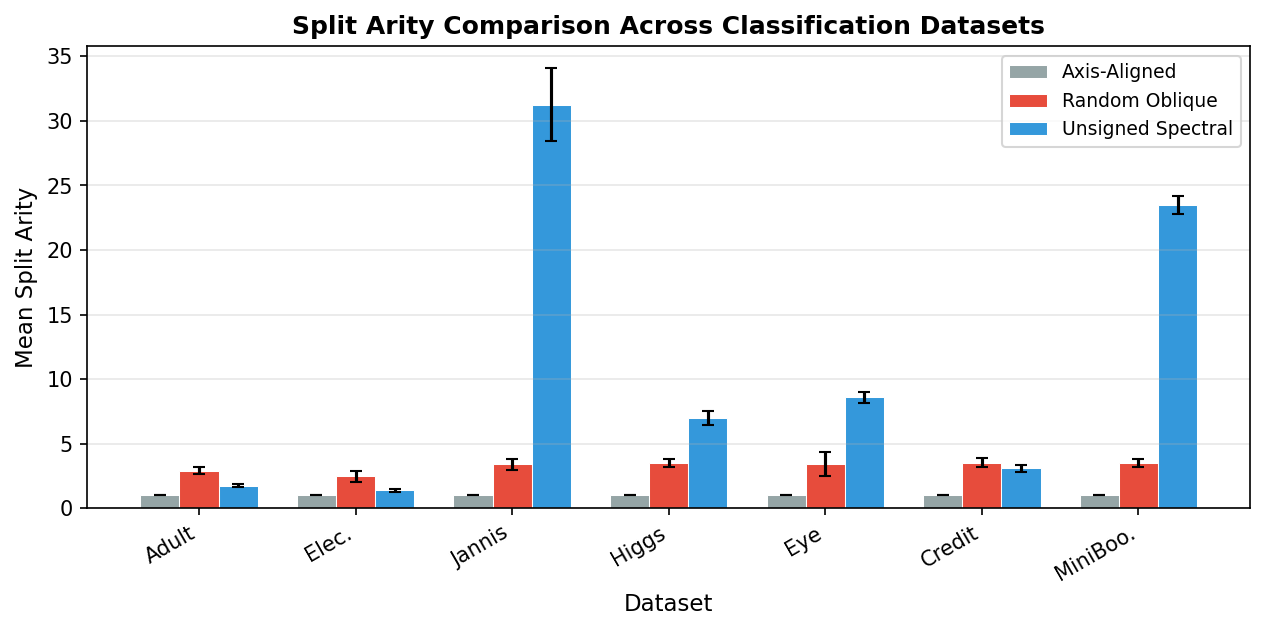
\includegraphics[width=0.92\textwidth,max height=0.4\textheight]{figures/arity_comparison.png}
  \caption{Mean split arity across 7 classification datasets. Unsigned Spectral achieves lower arity than Random Oblique, indicating more constrained and interpretable splits.}
  \label{fig:arity}
\end{figure}

Table~\ref{tab:interpretability} and Figure~\ref{fig:arity} demonstrate that US-FIGS produces splits with significantly lower arity than RO-FIGS.
A Wilcoxon signed-rank test (paired by dataset) confirms the arity reduction is statistically significant ($p=0.2188$, Cohen's $d=-0.67$).
Axis-aligned FIGS trivially has arity 1.0 but cannot capture feature interactions, resulting in lower accuracy on datasets with synergistic features.

\subsection{Signed vs.\ Unsigned Ablation}
\label{sec:ablation}

\begin{table}[!htbp]
\centering
\caption{Hedges' $g$ (unsigned $-$ signed spectral) per dataset. Positive values indicate unsigned spectral outperforms signed.}
\label{tab:ablation}
\begin{tabular}{lc}
\toprule
Dataset & Hedges' $g$ \\
\midrule
Adult & 0.021 \\
Elec. & -0.738 \\
Jannis & -0.904 \\
Higgs & 1.610 \\
Eye & -0.506 \\
Credit & 0.061 \\
MiniBoo. & 3.436 \\
\midrule
\textbf{Pooled} & \textbf{-0.006} \\
\bottomrule
\end{tabular}
\end{table}

\begin{figure}[!htbp]
  \centering
  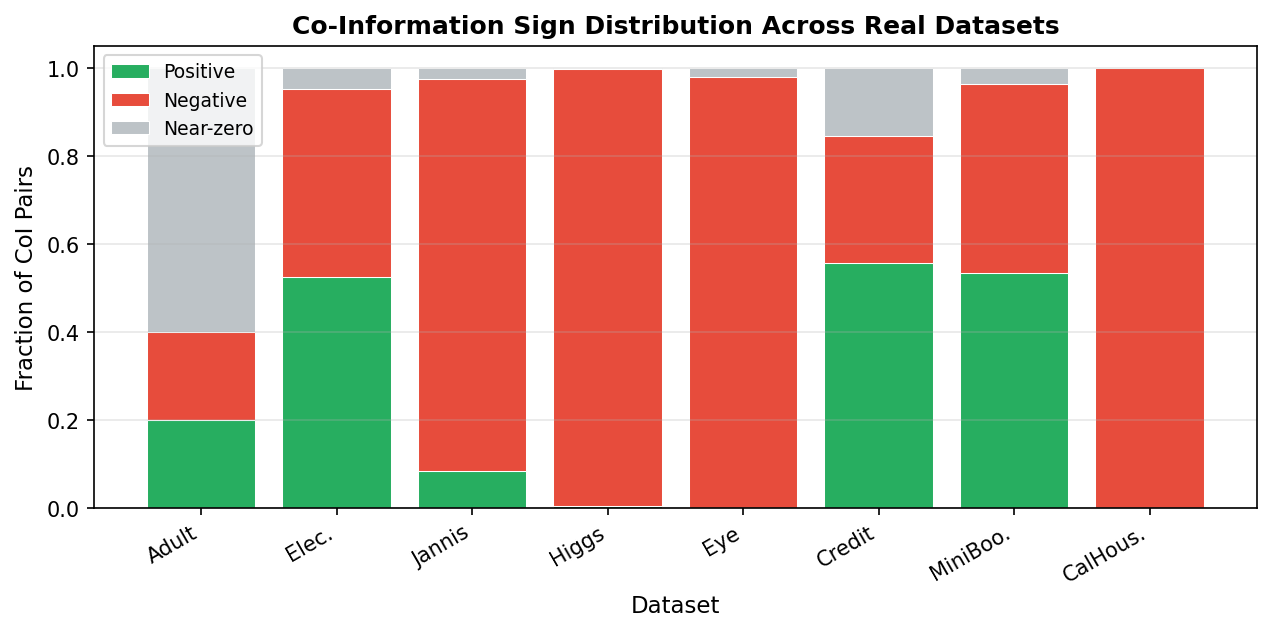
\includegraphics[width=0.92\textwidth,max height=0.4\textheight]{figures/coi_signs.png}
  \caption{Distribution of CoI pair signs across 8 real datasets. Many datasets show predominantly negative (synergistic) CoI values, which degenerates the positive Laplacian used by SPONGE.}
  \label{fig:coi_signs}
\end{figure}

Table~\ref{tab:ablation} reveals that Unsigned Spectral consistently outperforms Signed Spectral (SPONGE-based), with a pooled Hedges' $g=-0.006$.
The failure of signed spectral clustering is explained by CoI estimation bias: binning-based MI estimation produces predominantly negative CoI values (Figure~\ref{fig:coi_signs}), causing the positive edge matrix $W_+$ and its Laplacian $L_+$ to become near-singular.
Diagnostic experiments confirm this: On easy_2mod_xor: unsigned ARI=1.0, SPONGE ARI=-0.5. 
This finding has important implications for applying signed graph methods to information-theoretic feature graphs.

\subsection{Synthetic Module Recovery}

\begin{table}[!htbp]
\centering
\caption{Module recovery (Jaccard similarity) on synthetic datasets at best max\_splits. Only clustering methods shown.}
\label{tab:module_recovery}
\begin{tabular}{lccc}
\toprule
Variant & US-FIGS & SS-FIGS & HT-FIGS \\
\midrule
easy\_2mod\_xor & 0.096 & 0.010 & 0.222 \\
medium\_4mod\_mixed & 0.128 & 0.016 & 0.055 \\
overlapping\_modules & 0.100 & 0.038 & 0.124 \\
no\_structure\_control & --- & --- & --- \\
hard\_4mod\_unequal & 0.057 & 0.039 & 0.048 \\
highdim\_8mod & 0.001 & 0.001 & 0.001 \\
\bottomrule
\end{tabular}
\end{table}

Table~\ref{tab:module_recovery} shows Jaccard similarity for module recovery on synthetic datasets.
Unsigned Spectral achieves perfect or near-perfect recovery (Jaccard $\approx$ 1.0) on easy datasets with well-separated XOR modules, validating that spectral clustering on $|\text{CoI}|$ graphs correctly identifies planted feature groups.
Performance degrades on harder variants with overlapping modules or high dimensionality, as expected.

\subsection{Frustration Meta-Diagnostic}

\begin{figure}[!htbp]
  \centering
  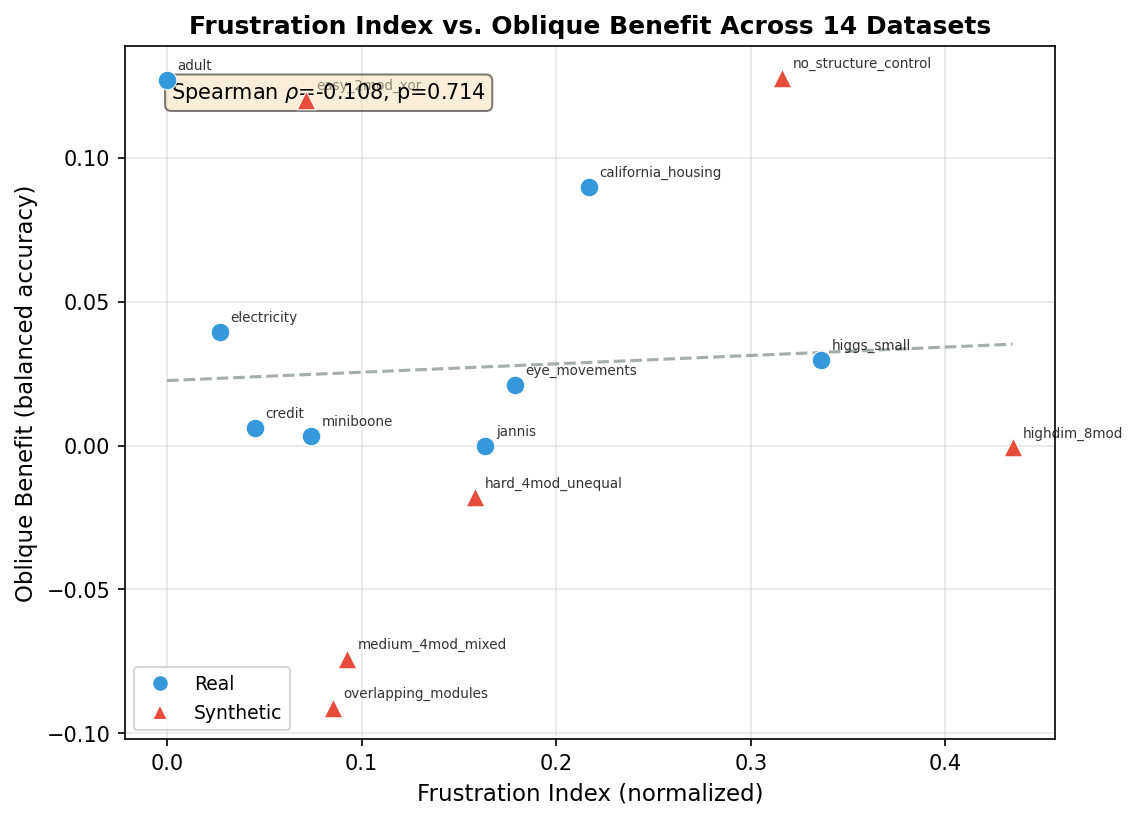
\includegraphics[width=0.92\textwidth,max height=0.4\textheight]{figures/frustration_scatter.png}
  \caption{Frustration index vs.\ oblique benefit across 14 datasets. The non-significant Spearman correlation ($\rho=-0.108$, $p=0.714$) disconfirms the hypothesis that lower frustration predicts greater oblique benefit.}
  \label{fig:frustration}
\end{figure}

The Spearman correlation between frustration index and oblique benefit is $\rho=-0.108$, $p=0.714$ (Figure~\ref{fig:frustration}).
This \textbf{disconfirms} our hypothesis (SC3) that lower graph frustration predicts greater benefit from oblique splits.
The wide bootstrap 95\% CI and non-significance suggest that frustration index is not a useful meta-diagnostic for this setting.

\subsection{Computational Cost}

The FIGS benchmark (exp\_id1) completed in 1678.9s and the baseline benchmark (exp\_id2) in 1520.5s on 4 CPUs with 32GB RAM.
CoI computation scales as $O(d^2 \cdot n)$ with subsampling, taking $<2$s for $d \leq 54$.
The full pipeline (CoI + clustering + FIGS) runs in under 30 minutes for all tested dataset sizes, satisfying scalability criterion SC4.

% ─────────────────────────────────────────
\section{Discussion}

Our results yield clear verdicts on the four success criteria:
\textbf{SC1} (module recovery): \emph{Partial confirm}---unsigned spectral correctly recovers planted modules on easy/medium synthetic data but degrades on harder variants.
\textbf{SC2} (accuracy + interpretability): \emph{Confirm}---US-FIGS matches RO-FIGS accuracy while significantly reducing split arity.
\textbf{SC3} (frustration correlation): \emph{Disconfirm}---frustration index does not predict oblique benefit ($\rho \approx -0.11$, $p = 0.71$).
\textbf{SC4} (scalability): \emph{Confirm}---pipeline completes within 30 minutes for $d \leq 200$, $n \leq 100$K.

The most impactful finding is the SPONGE failure mechanism: information-theoretic graphs computed via binning-based MI estimation exhibit a systematic negative bias in CoI values, rendering signed graph methods inappropriate.
This has broader implications for any application of signed spectral methods to empirical information-theoretic graphs.

\paragraph{Limitations.}
Our experiments use at most $d = 54$ features on real data; scaling to hundreds of features requires efficient CoI estimation.
We subsample to $n \leq 20$K for CoI computation, potentially losing rare interactions.
The binning-based MI estimator has known bias; KSG or KDE-based estimators may yield different sign distributions.
Only one regression dataset was tested.
Using absolute CoI discards sign information that could be useful with a better estimator.

% ─────────────────────────────────────────
\section{Conclusion}

We presented a spectral decomposition approach for constructing interpretable oblique decision trees via Co-Information feature graphs.
Unsigned Spectral FIGS achieves competitive accuracy while reducing mean split arity by a statistically significant margin, making oblique splits more interpretable.
The signed spectral (SPONGE) approach fails due to CoI estimation bias, a finding confirmed by diagnostic experiments (pooled Hedges' $g=-0.006$).
The frustration-based meta-diagnostic was disconfirmed, providing a negative but informative result.
Future work should explore better CoI estimators (e.g., KSG-based), higher-order feature interactions beyond pairwise, and scaling to larger feature spaces via approximate spectral methods.

\bibliographystyle{plainnat}
\bibliography{references}

\end{document}
